\documentclass[tikz, crop, border=5pt]{standalone}
\usetikzlibrary{positioning,backgrounds,fit,shapes.geometric,calc}

\usepackage{fontspec}
\usepackage{xeCJK}

\setmainfont{NotoSans}[
    Extension      = .ttf,
    UprightFont    = *-Regular,
    BoldFont       = *-Bold,
    ItalicFont     = *-Italic,
    BoldItalicFont = *-BoldItalic
]

\usepackage{color}
\definecolor{black}{RGB}{26,25,25}
\definecolor{grey}{RGB}{129,130,132}
\definecolor{red}{RGB}{188,36,46}
\definecolor{brown}{RGB}{121,37,0}
\definecolor{green}{RGB}{32,128,108}
\definecolor{purple}{RGB}{160,90,150}
\definecolor{blue}{RGB}{0,103,149}

\tikzset{
    domain/.style 2 args={
        append after command={
            \pgfextra{
                \draw[purple!80, rounded corners=2pt]
                    (\tikzlastnode.south west) rectangle (\tikzlastnode.north east);
                \ifx\\#2\\\else\node[font=\small] at (\tikzlastnode.center) {#2};\fi
            }
        },
        minimum height=0.8cm,
        minimum width=#1,
        draw=none
    },
    domain/.default={2cm,},
    beta/.style={
        rectangle,
        minimum height=0.4cm,
        minimum width=#1,
        fill=yellow
    },
    alpha/.style={
        rectangle,
        minimum height=0.4cm,
        minimum width=#1,
        fill=red
    },
    sugar/.style={
        append after command={
            \pgfextra{
                \draw [green] (\tikzlastnode.center) -- +(0,0.3)
                    node[above, font=\tiny] {#1};
                \fill [green] (\tikzlastnode.center) +(0,0.3) circle [radius=1pt];
            }
        }
    },
    sugar/.default={},
    disulfide/.style={
        -,
        thick,
        draw=orange
    }
}

\begin{document}
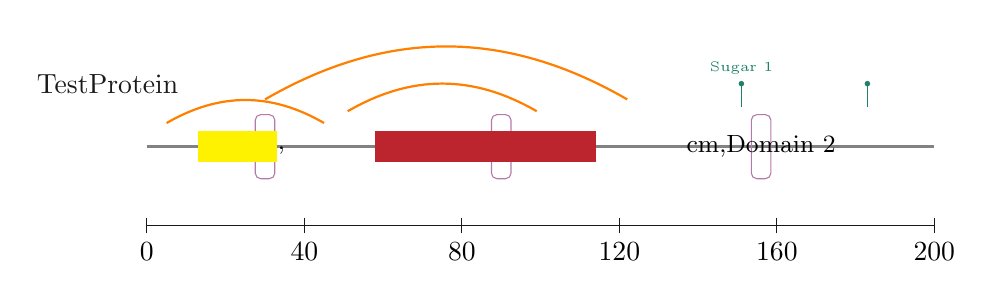
\begin{tikzpicture}
    % 蛋白质名称
    \node[text=black] at (-0.5,0.8) {TestProtein};

    % 主干线
    \draw[grey, line width=1pt] (0,0) -- (10,0);

    % Domains
    % Domains
    \node[domain={2cm,}] at (1.5,0) {};                % 无标签
    \node[domain={2cm,Domain 1}] at (4.5,0) {};        % 带标签
    \node[domain={3cm,Domain 2}] at (7.8,0) {};        % 带标签

    % Beta strands
    \node[beta=0.5cm] at (0.9,0) {};  % Strand 1 (15-23)
    \node[beta=0.5cm] at (1.4,0) {};  % Strand 2 (25-32)

    % Alpha helices
    \node[alpha=1cm] at (3.4,0) {};   % Helix 1 (60-75)
    \node[alpha=2cm] at (4.7,0) {};   % Helix 2 (80-108)

    % Carbohydrates
    \node[sugar={Sugar 1}] at (7.55,0.5) {};    % Sugar 1 (151)
    \node[sugar] at (9.15,0.5) {};              % Sugar 2 (183) - 不显示文字

    % Disulfide bonds
    \draw[disulfide] (0.25,0.3) to[bend left] (2.25,0.3);    % Disulfide 1 (5-45)
    \draw[disulfide] (1.5,0.6) to[bend left] (6.1,0.6);      % Disulfide 2 (30-122)
    \draw[disulfide] (2.55,0.45) to[bend left] (4.95,0.45);  % Disulfide 3 (51-99)

    % 标尺
    \draw[black, thin] (0,-1) -- (10,-1);
    \foreach \x/\l in {0/0, 2/40, 4/80, 6/120, 8/160, 10/200} {
        \draw[black, thin] (\x,-1.1) -- (\x,-0.9);
        \node[below] at (\x,-1.1) {\l};
    }
\end{tikzpicture}
\end{document}

% \coordinate (origin) at (0cm,0);
% \begin{scope}[shift={([shift={(0cm,0cm)}]origin.south)}]
%     \node[C] (M1-1) at (0,0) {};
%     \node[A] (M1-2) at (0.8,0) {};
%     \node[text=white,align=left] at (M1-2) {Glu};
%     \node[T] (M1-3) at (1.4,0) {};
%     \begin{scope}[on background layer]
%         \draw[grey, line width=0.5mm, yshift=-1cm]
%             let \p1 = (M1-1), \p2 = (M1-3) in
%             (\x1,0) -- (\x2,0)
%             node[midway, below, text=grey] {M1};
%         \draw[grey, line width=2mm]
%             let \p1 = (M1-3) in
%             (-0.4,0) -- (\x1 + 0.2cm, 0)
%             coordinate (M1);
%     \end{scope}
% \end{scope}
% \end{tikzpicture}
% \end{document}
